% !TeX root = ../main.tex

\chapter{系统需求分析}

需求分析是软件生产周期中的一个重要环节,本章将采用面向对象分析的方法对体系结构模拟器的需求进行具体分析与建模。明确模拟器所需实现的功能性需求和非功能性需求。

\section{需求导出}

在芯片设计及验证的流程中,对于基础系统软件尤其是操作系统,底层驱动等的适配和验证往往是反馈硬件设计缺陷最频繁的部分,这部分的工作不仅是对于前期硬件设计的重要测试,也是后续用户态程序开发的基础。对于系统软件的移植和适配工作,有两种主流方式,一种是在模拟芯片硬件特性的FPGA开发板上仿真,另一种是通过软件模拟。两种方法各有利弊,FPGA开发板更加接近真实硬件环境,能够获取精确的仿真信号,但是速度相对较慢,并且能够提供的调试信息较少。而模拟器环境下的开发,其运行速度接近宿主机,并且调试方便,虽然信号精度与真实硬件有差异,但是能够在测试的前期反馈大部分的缺陷。所以真实的开发和测试流程一般是先使用模拟器验证,再上FPGA平台仿真,这样既能够提高开发效率,又不失精度。
随着RISC-V开源社区的日益壮大,更多的芯片设计厂商选择RISC-V作为其指令集架构,在芯片的验证过程中,软硬件适配工作作为测试的重点,往往需要模拟器环境的支持。当前RISC-V开源社区提供的模拟器作为教学工具可以帮助的初学者快速上手,但是对于实际的芯片开发团队来说,系统软件的移植和开发工作需要一款符合实际硬件设计的模拟器,对真实的硬件功能进行模拟,同时要能够提供强大的调试工具,方便系统软件的开发迭代。本模拟器主要用于芯片开发项目后期的验证工作和系统软件移植工作,对于一些具体的硬件细节,如流水线,分支预测等不进行模拟,只对处理器功能进行模拟,属于解释型的指令集模拟器。


\section{分析建模}

指令集模拟器的主要参与者是进行系统软件开发和移植的程序员,
首先使用RISC-V交叉编译工具链将目标程序编译为RISC-V架构的ELF文件,然后模拟器解析该elf文件,将对应的指令流搬运到bootrom,模拟器在配置启动后为处理器注册指令集,绑定解码器,逐条进行译码,执行。指令译码器完成包括操作数在内的指令信息提取,找到该条指令注册时对应的功能函数,执行该功能函数,然后将更新后的寄存器状态信息,内存状态信息同步到前端UI显示模块。在模拟器运行的过程中,用户还可以通过前端交互调试窗口来切换模拟器运行模式,设置断点触发条件,进行单步调试,状态查询等操作。
通过对实际芯片开发验证过程的分析和归纳,得出模拟器所需要的主要功能有:


1) 设置模拟器启动配置,包括elf文件路径添加,指令集模块注册,运行模式选择等。


2) 模拟器执行流程控制。包括正常运行模式下的uart串口交互,暂停执行进入调试模式,模拟器重启。


3) 调试功能。在调试模式下,进行断点设置,内存查询,历史指令查询,单步执行等。


4) 模拟外部中断信号发送。


综上所述,用户需求描述表如表~\ref{tab:tab1}所示。
\begin{table}[H]
  \centering
  \caption{用户需求描述表}
  \label{tab:tab1}
  \renewcommand\arraystretch{1.2}
  \begin{tabular}{ccl}
    \toprule
    名称   & 参与者   & 说明   \\
    \midrule
    模拟器配置并启动 & 系统软件开发/移植程序员 & \multicolumn{1}{p{5cm}}{设置模拟器启动参数并运行} \\ \hline
    切换至调试模式 &	系统软件开发/移植程序员	& \multicolumn{1}{m{5cm}}{模拟器从运行模式切换为调试模式}\\
    \hline
    切换至运行模式 & 系统软件开发/移植程序员	& \multicolumn{1}{m{5cm}}{模拟器从调试模式切换为运行模式}\\
    \hline
    重启模拟器	& 系统软件开发/移植程序员	& \multicolumn{1}{p{5cm}}{重新加载当前配置项并运行}\\
    \hline
    断点设置 &	系统软件开发/移植程序员 &	\multicolumn{1}{p{5cm}}{调试模式下进行断点添加/移除}\\
    \hline
    内存查询 &	系统软件开发/移植程序员 &	\multicolumn{1}{m{5cm}}{调试模式下对虚拟地址/物理地址内容查询}\\
    \hline
    中断信号发送	& 系统软件开发/移植程序员 &	\multicolumn{1}{m{5cm}}{点击外部中断源按钮,发送对应的外部中断到plic}\\
    \bottomrule
  \end{tabular}
\end{table}


根据用例描述表可以得出系统软件开发/移植程序员的用例图如图~\ref{fig:use-case}所示。
\begin{figure}[H]
  \centering
  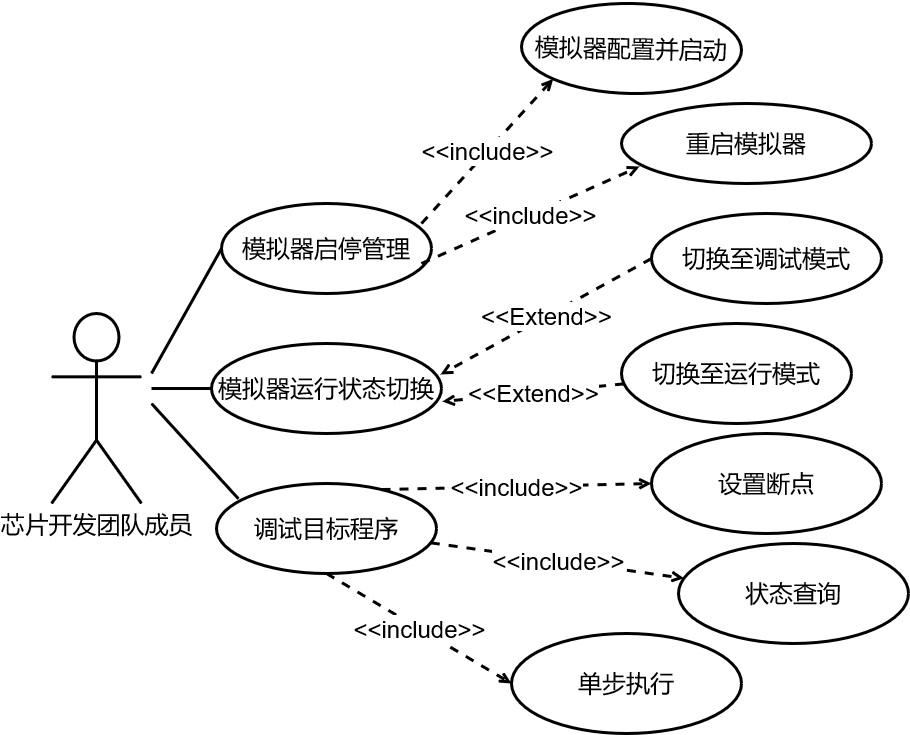
\includegraphics[width=0.9\textwidth]{use-case.png}
  \caption{系统软件开发/移植人员用例图}
  \label{fig:use-case}
\end{figure}


下面分别对系统软件开发/移植程序员的五个主要用例进行详细描述。 


模拟器配置启动的用例描述如表~\ref{tab:yongli1}所示。
\begin{table}[H]
  \centering
  \caption{模拟器配置启动用例描述}
  \label{tab:yongli1}
  \renewcommand\arraystretch{1.1}
  \begin{tabular}{cl}
    \toprule
用例名称 &	模拟器配置启动\\
    \midrule
用例描述 &	设置模拟器启动参数并运行\\ \hline
触发条件 &	勾选模拟器配置选项,输入elf文件路径\\ \hline
后置条件 &	模拟器解析配置参数,启动程序\\ \hline
	& (1)	输入elf文件路径 \\
  基本事件流 & (2)	选择启动模式是否为调试模式 \\
 & (3)	其他参数勾选,包括核心数,模拟外设路径等\\ \hline
异常事件流	& 配置参数错误,启动失败\\
    \bottomrule
  \end{tabular}
\end{table}


模拟器切换调试模式用例描述如表~\ref{tab:yongli2}所示。
\begin{table}[H]
  \centering
  \caption{切换调试模式用例描述}
  \label{tab:yongli2}
  \renewcommand\arraystretch{1.1}
  \begin{tabular}{cl}
    \toprule
用例名称	& 切换调试模式\\
    \midrule
用例描述	& 模拟器从运行模式切换为调试模式\\ \hline
触发条件	& 点击run/stop按键\\ \hline
后置条件	& 模拟器进入调试模式/模拟器进入运行模式\\ \hline
基本事件流	& 在运行模式下点击run/stop按键\\ \hline
异常事件流	& 运行模式下点击run按键/调试模式下点击halt按键\\
    \bottomrule
  \end{tabular}
\end{table}


模拟器断点设置的用例描述如表~\ref{tab:yongli3}所示。
\begin{table}[H]
  \centering
  \caption{断点设置用例描述}
  \label{tab:yongli3}
  \renewcommand\arraystretch{1.1}
  \begin{tabular}{cl}
    \toprule
用例名称	& 断点设置\\
    \midrule
用例描述	& \multicolumn{1}{p{9cm}}{调试模式下进行断点添加/移除}\\ \hline
触发条件	& \multicolumn{1}{m{9cm}}{在调试窗口勾选断点类型,输入断点条件,点击”应用”}\\ \hline
后置条件	& \multicolumn{1}{m{9cm}}{点击run进入运行模式,模拟器运行至断点条件触发调试中断,进入调试模式}\\ \hline
 & \multicolumn{1}{m{9cm}}{(1)	调试窗口添加/移除断点}\\
 基本事件流 & \multicolumn{1}{m{9cm}}{(2)	程序运行,触发断点}\\
 & \multicolumn{1}{m{9cm}}{(3)	进入调试模式,打印断点信息}\\ \hline
异常事件流	& \multicolumn{1}{m{9cm}}{断点信息填写错误导致无效断点条件}\\
    \bottomrule
  \end{tabular}
\end{table}


模拟器内存查询的用例描述如表~\ref{tab:yongli4}所示。
\begin{table}[H]
  \centering
  \caption{内存查询用例描述}
  \label{tab:yongli4}
  \renewcommand\arraystretch{1.1}
  \begin{tabular}{cl}
    \toprule
用例名称	& 内存查询\\
    \midrule
用例描述	& 调试模式下对虚拟地址/物理地址内容查询\\ \hline
触发条件	& 查询窗口输入内存地址,点击查询\\ \hline
后置条件	& 输出内存对应地址内容\\ \hline
	& (1) 选择地址类型为虚拟地址/物理地址\\
  基本事件流 &            (2) 虚拟地址需要指定核心id\\
 &            (3) 输入16进制地址,点击查询\\ \hline
异常事件流	& 输入无效地址导致访存失败\\
    \bottomrule
  \end{tabular}
\end{table}


模拟器mailbox中断信号发送的用例描述如表~\ref{tab:yongli5}所示。
\begin{table}[H]
  \centering
  \caption{mailbox中断信号发送用例描述}
  \label{tab:yongli5}
  \renewcommand\arraystretch{1.1}
  \begin{tabular}{cl}
    \toprule
用例名称 & mailbox中断信号发送\\
    \midrule
用例描述	& 点击外部中断源按钮,发送对应的外部中断到plic\\ \hline
触发条件	& 点击对应中断源的中断信号发送按键\\ \hline
后置条件	& 模拟器响应中断,执行中断处理程序\\ \hline
 &	(1)	点击mailbox中断源发送中断信号\\
 基本事件流 & (2)	弹出mailbox消息窗口,填写消息,点击发送\\
 & (3)	系统接受外部中断,执行自定义的中断处理函数,显示在mailbox窗口\\ \hline
异常事件流 &	mailbox中断发送后系统无响应\\
    \bottomrule
  \end{tabular}
\end{table}


\section{非功能性需求}

该指令集模拟器的非功能性需求有:


(1) 准确性: 体系结构模拟器的首要需求就是准确性,只有准确模拟出真实硬件的行为,才能在模拟器上进行后续的软件开发和移植工作。由于本模拟器的模拟精度在指令级别,不涉及到流水线,乱序执行,分支预测等更细粒度的模拟,因此要求模拟器要和真实硬件在寄存器级别完全一致。


(2) 可靠性: 可靠性要求模拟器要能够在使用过程中持续稳定运行,不会因为宿主机上程序的设计缺陷导致模拟过程发生崩溃。如果遇到异常情况,模拟器需要能够在不修改启动配置的情况下重启成功,且模拟过程是可复现的。


(3) 实时性: 作为一个基于指令集翻译的体系结构模拟器,虽然本身的设计初衷不是为了测试CPU性能,但是模拟器运行速度至少需要达到10MIPS。


(4) 友好性: 模拟器需要提供一个结构清晰的可视化界面,调试模式下需要能够及时更新处理器状态,包括寄存器值,历史汇编指令列表等。需要提供便捷的内存查询功能,外部中断模拟发送等。




\section{本章小结}

本章主要是采用面向对象分析的方法,在实际的芯片开发项目过程中,对系统软件移植/开发/测试流程进行剖析,确定了指令集模拟器需要实现的功能以及其他的非功能性需求,最终形成了系统的需求规格说明书,为后续的系统概要设计,具体实现以及最后的系统测试工作奠定了基础.


